%-------------------------------------------------------------------------------
\section{Evaluation}
\label{s:eval}
%-------------------------------------------------------------------------------

We begin by evaluating the existing alternatives to \cgroups{} that currently
exist in Linux in \autoref{ss:eval:existing}. We then explore the performance of
\schedbe{} in relation to the following questions:
\begin{enumerate}
    \item Does the new \schedbe{} isolate LC from BE workloads?
    \item Is parking necessary?
    \item How much does the patch cost?
\end{enumerate}

All the graphs in this paper run on Linux version 6.14.2, the baseline version
that our patch builds on.

\subsection{Existing approaches}\label{ss:eval:existing}

To show the benefits of \schedbe{}, we compare with existing alternatives within
Linux. The first is real time scheduling, because this is a place where Linux
already enforces categorical global priorities: processes that run in real time
have strict priority over other processes. The second is the existing mechansism
of \schedidle{}, which \schedbe{} is based on.

\subsubsection{Realtime scheduling}

Linux enforces the categorical separation of real time tasks by using
\textit{scheduling classes}. Each scheduling class exists completely separately:
classes maintain their own runqueues and per-entity state; implement their own
scheduling algorithms to choose from the entities on their runqueue; and balance
the load across runqueues on different cores.

Linux isolates strictly between different scheduling classes: it only schedules
a lower scheduling class if the higher scheduling classes found nothing to run,
and each scheduling class tries to steal work from other cores before returning
that it has nothing to run --- these two checks represent the entry and exit
synchronization points. It is thereby true that if something in the Normal
scheduling class is running, it means there are no Fifo tasks waiting to run
anywhere on the machine.

This points to a possible alternative: run LC in the Fifo scheduling class and BE
in Normal.\footnote{The Deadline scheduling class is not a good fit, since it
requires accurate knowledge of a processes runtime (processing time per request)
and period (when requests come in)} Fifo runs a priority scheduler: it has 99
priorities, each takes strict precedent over the one lower; within priorities
the scheduler enforces a global first-in-first-out (hence the Fifo class name),
based on when processes become runnable.

\begin{figure}[t]
    \centering
    \begin{subfigure}[t]{0.48\columnwidth}
        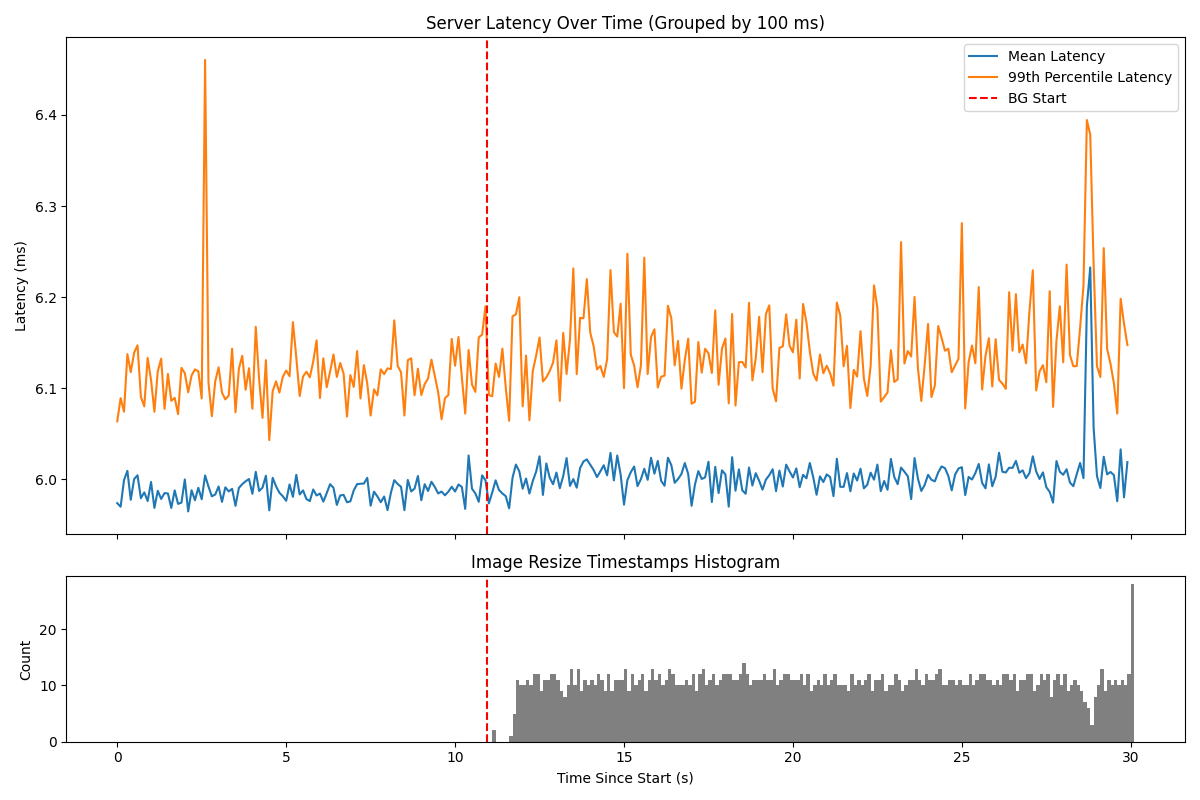
\includegraphics[width=\columnwidth]{graphs/srv-bg-rt-low.png}
        \caption{Low load}\label{fig:srv-bg-rt-low}
    \end{subfigure}
    \hspace{\fill}
    \begin{subfigure}[t]{0.48\columnwidth}
        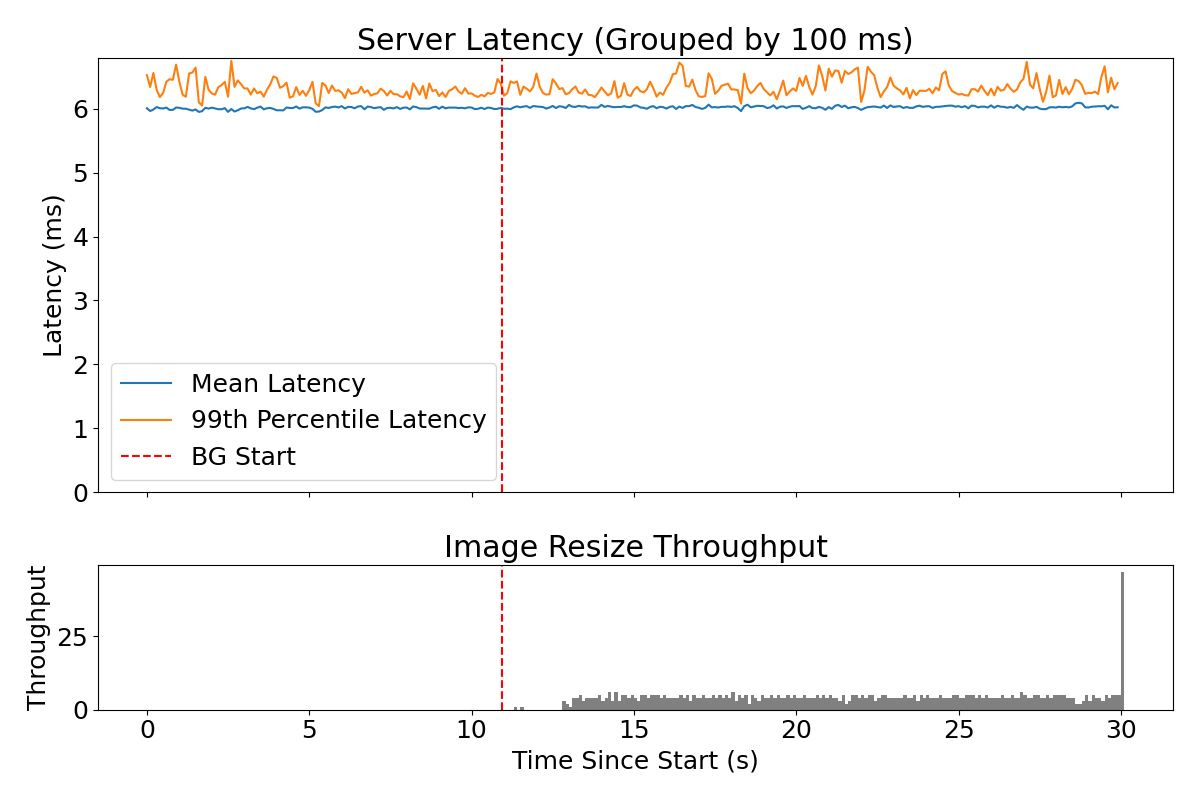
\includegraphics[width=\columnwidth]{graphs/srv-bg-rt-high.png}
        \caption{High load}\label{fig:srv-bg-rt-high}
    \end{subfigure}
    \vspace{4pt}
    \caption{Results of the same experiment, with LC running as a real time process}\label{fig:srv-bg-rt}
\end{figure}

We run the same experiment as in \autoref{s:intro}, but put the LC task in the
Fifo scheduling class, and leave BE tasks with the default process weight.
\autoref{fig:srv-bg-rt} shows the resulting measured latencies in the same low
and high load setting as previously. As expected, we see that Linux is able to
isolate the two very well. 

However, this is an untenable solution because of Fifo's run-to-completion
scheduling, which is known to have a failure mode of head-of-line (HoL) blocking
under varied request processing times, where long-running requests monopolize
the CPU while short requests wait in the queue. The Fifo scheduler also enforces
not only cross-core isolation between different priorities, but also a global
ordering within the same priority.

The takeaway is that Linux's current mechanism of scheduling classes can isolate
workloads effectively, but existing scheduling classes use scheduling
algorithms that are not a good fit for modern workloads.

\subsubsection{\schedidle}\label{ss:schedidle}

\schedidle{} is a scheduling \textit{policy}. Policies are not full scheduling
classes, but allow for special casing within a scheduling class. As we discussed
in \autoref{s:maybe-solution}, \schedidle{} is special cased, but only on
wakeup.\hmng{I took out the insight/connection that \schedidle{} is half a
scheduling class and \schedbe{} is/makes it a whole one because I didn't feel
like it fit here, but now I'm not sure where it does}

\begin{figure}[t]
    \centering
    \begin{subfigure}[t]{0.49\columnwidth}
        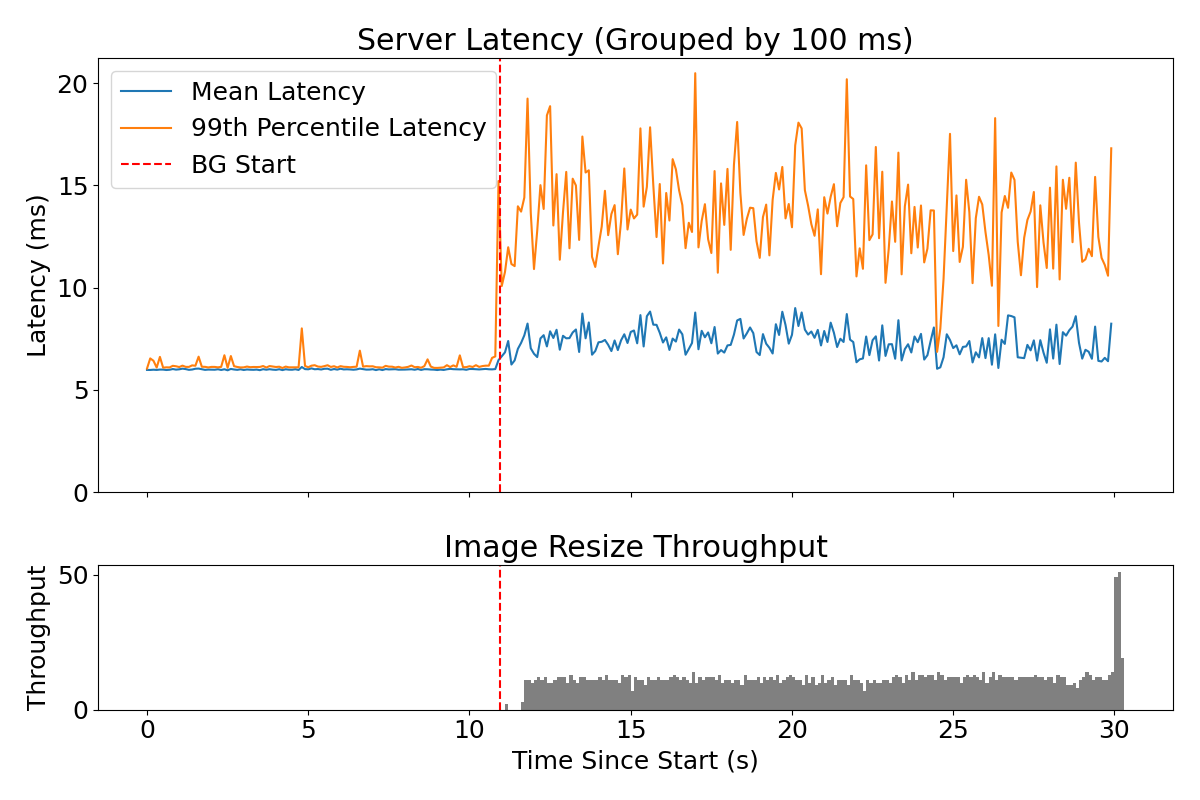
\includegraphics[width=\columnwidth]{graphs/srv-bg-idle-low.png}
        \caption{Low load}\label{fig:srv-bg-idle-low}
    \end{subfigure}
    \hspace{\fill}
    \begin{subfigure}[t]{0.49\columnwidth}
        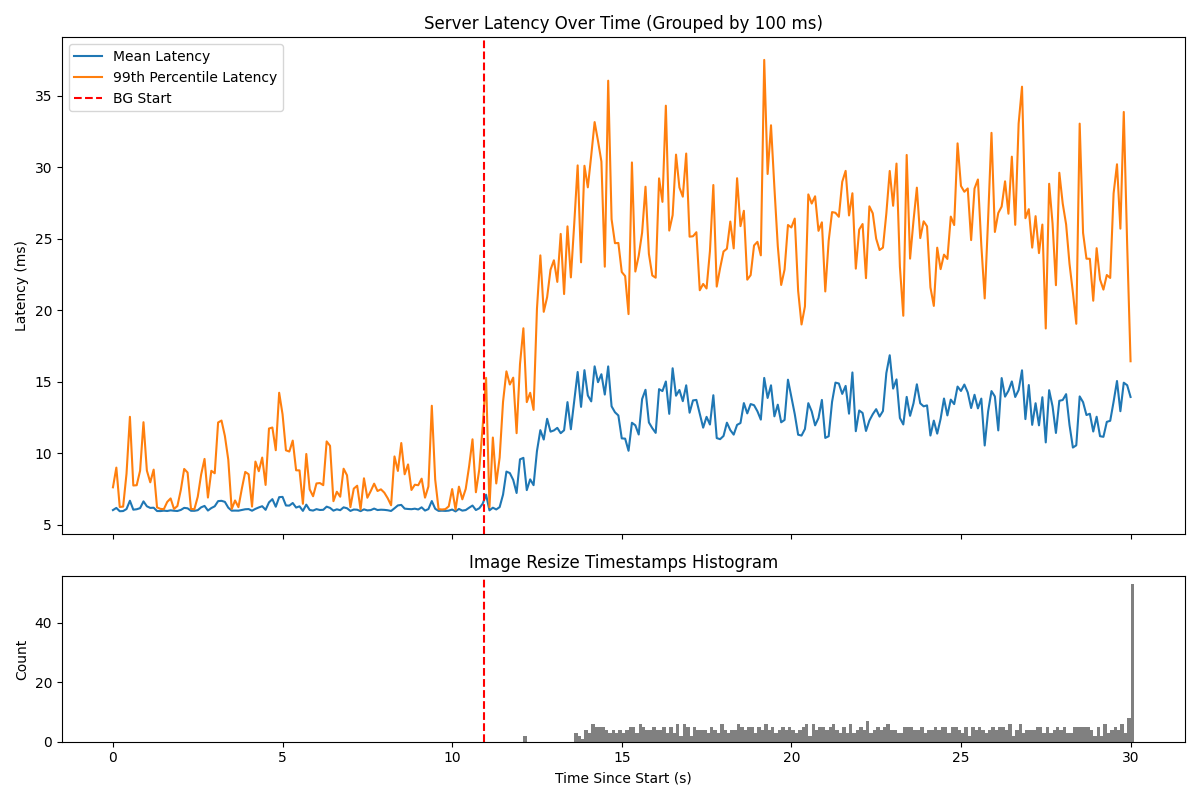
\includegraphics[width=\columnwidth]{graphs/srv-bg-idle-high.png}
        \caption{High load}\label{fig:srv-bg-idle-high}
    \end{subfigure}
    \vspace{4pt}
    \caption{using \schedidle{}}\label{fig:srv-bg-idle}
\end{figure}

And indeed, we find that when we use cgroups' new cpu.idle interface feature,
the latency impact of the BE tasks decreases, although it does not entirely drop
to what we saw with the Fifo class.\ \autoref{fig:srv-bg-idle} shows the
results, for the familiar settings of low and high load. The jump we see in the
mean latency has decreased from peaks as high as 20ms to around 8ms.

\subsection{Does \schedbe{} isolate?}

\begin{figure}[t]
    \centering
    \begin{subfigure}[t]{0.49\columnwidth}
        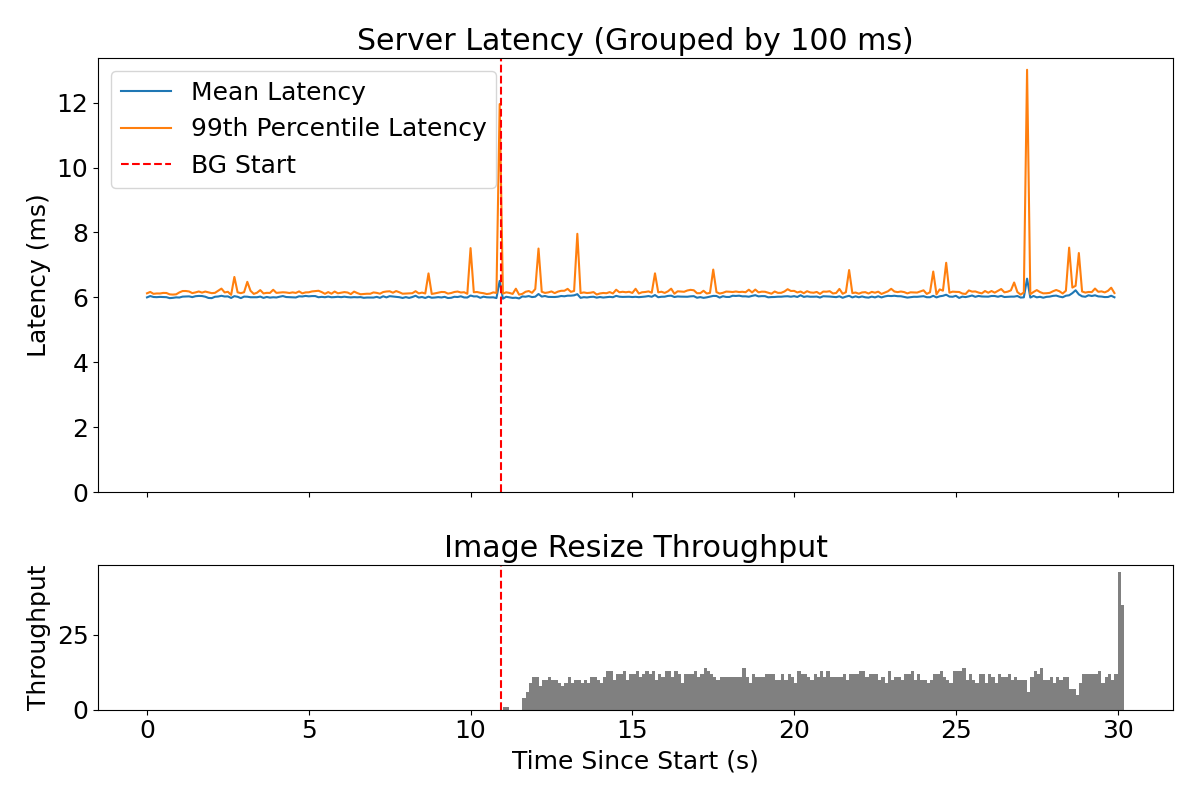
\includegraphics[width=\columnwidth]{graphs/srv-bg-schedbe-low.png}
        \caption{Low load}\label{fig:srv-bg-schedbe-low}
    \end{subfigure}
    \hspace{\fill}
    \begin{subfigure}[t]{0.49\columnwidth}
        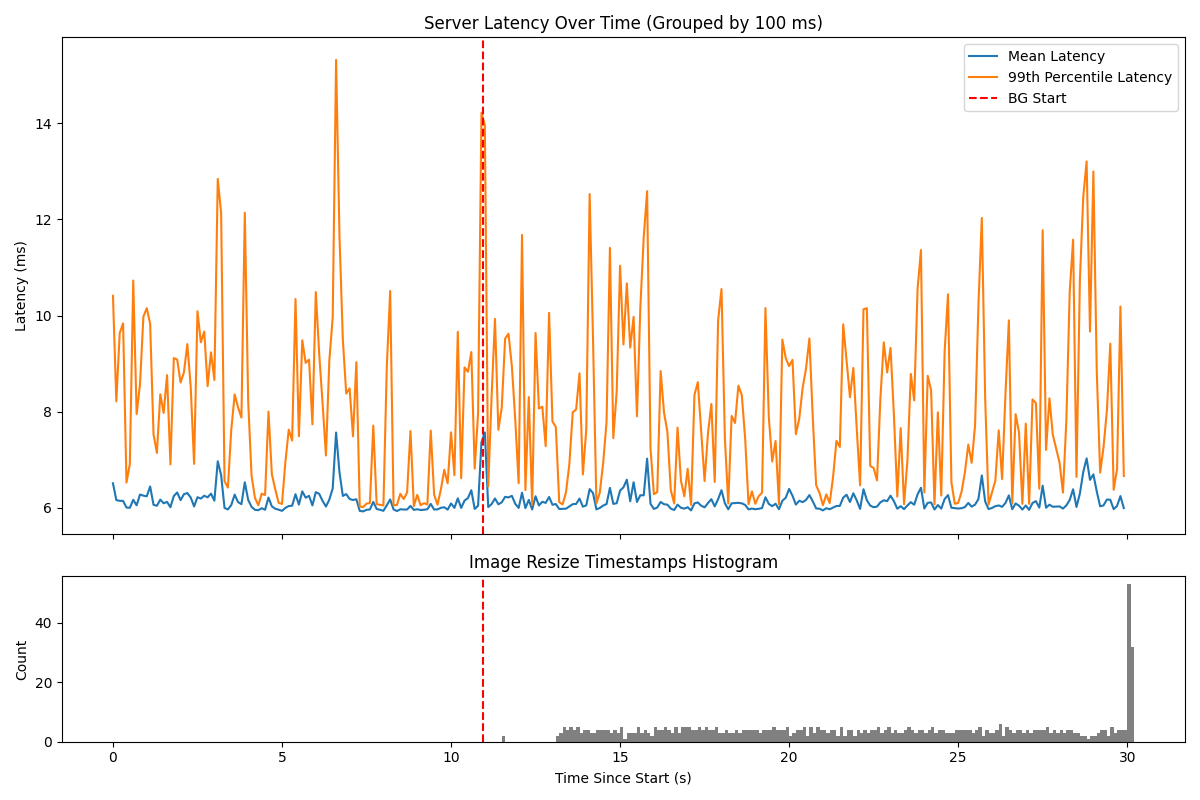
\includegraphics[width=\columnwidth]{graphs/srv-bg-schedbe-high.png}
        \caption{High load}\label{fig:srv-bg-schedbe-high}
    \end{subfigure}
    \vspace{4pt}
    \caption{using a patched \schedidle{} that steals queued \schednormal{}
    tasks before running \schedidle{} ones}\label{fig:srv-bg-schedbe}
\end{figure}

\begin{figure}[t]
    \centering
    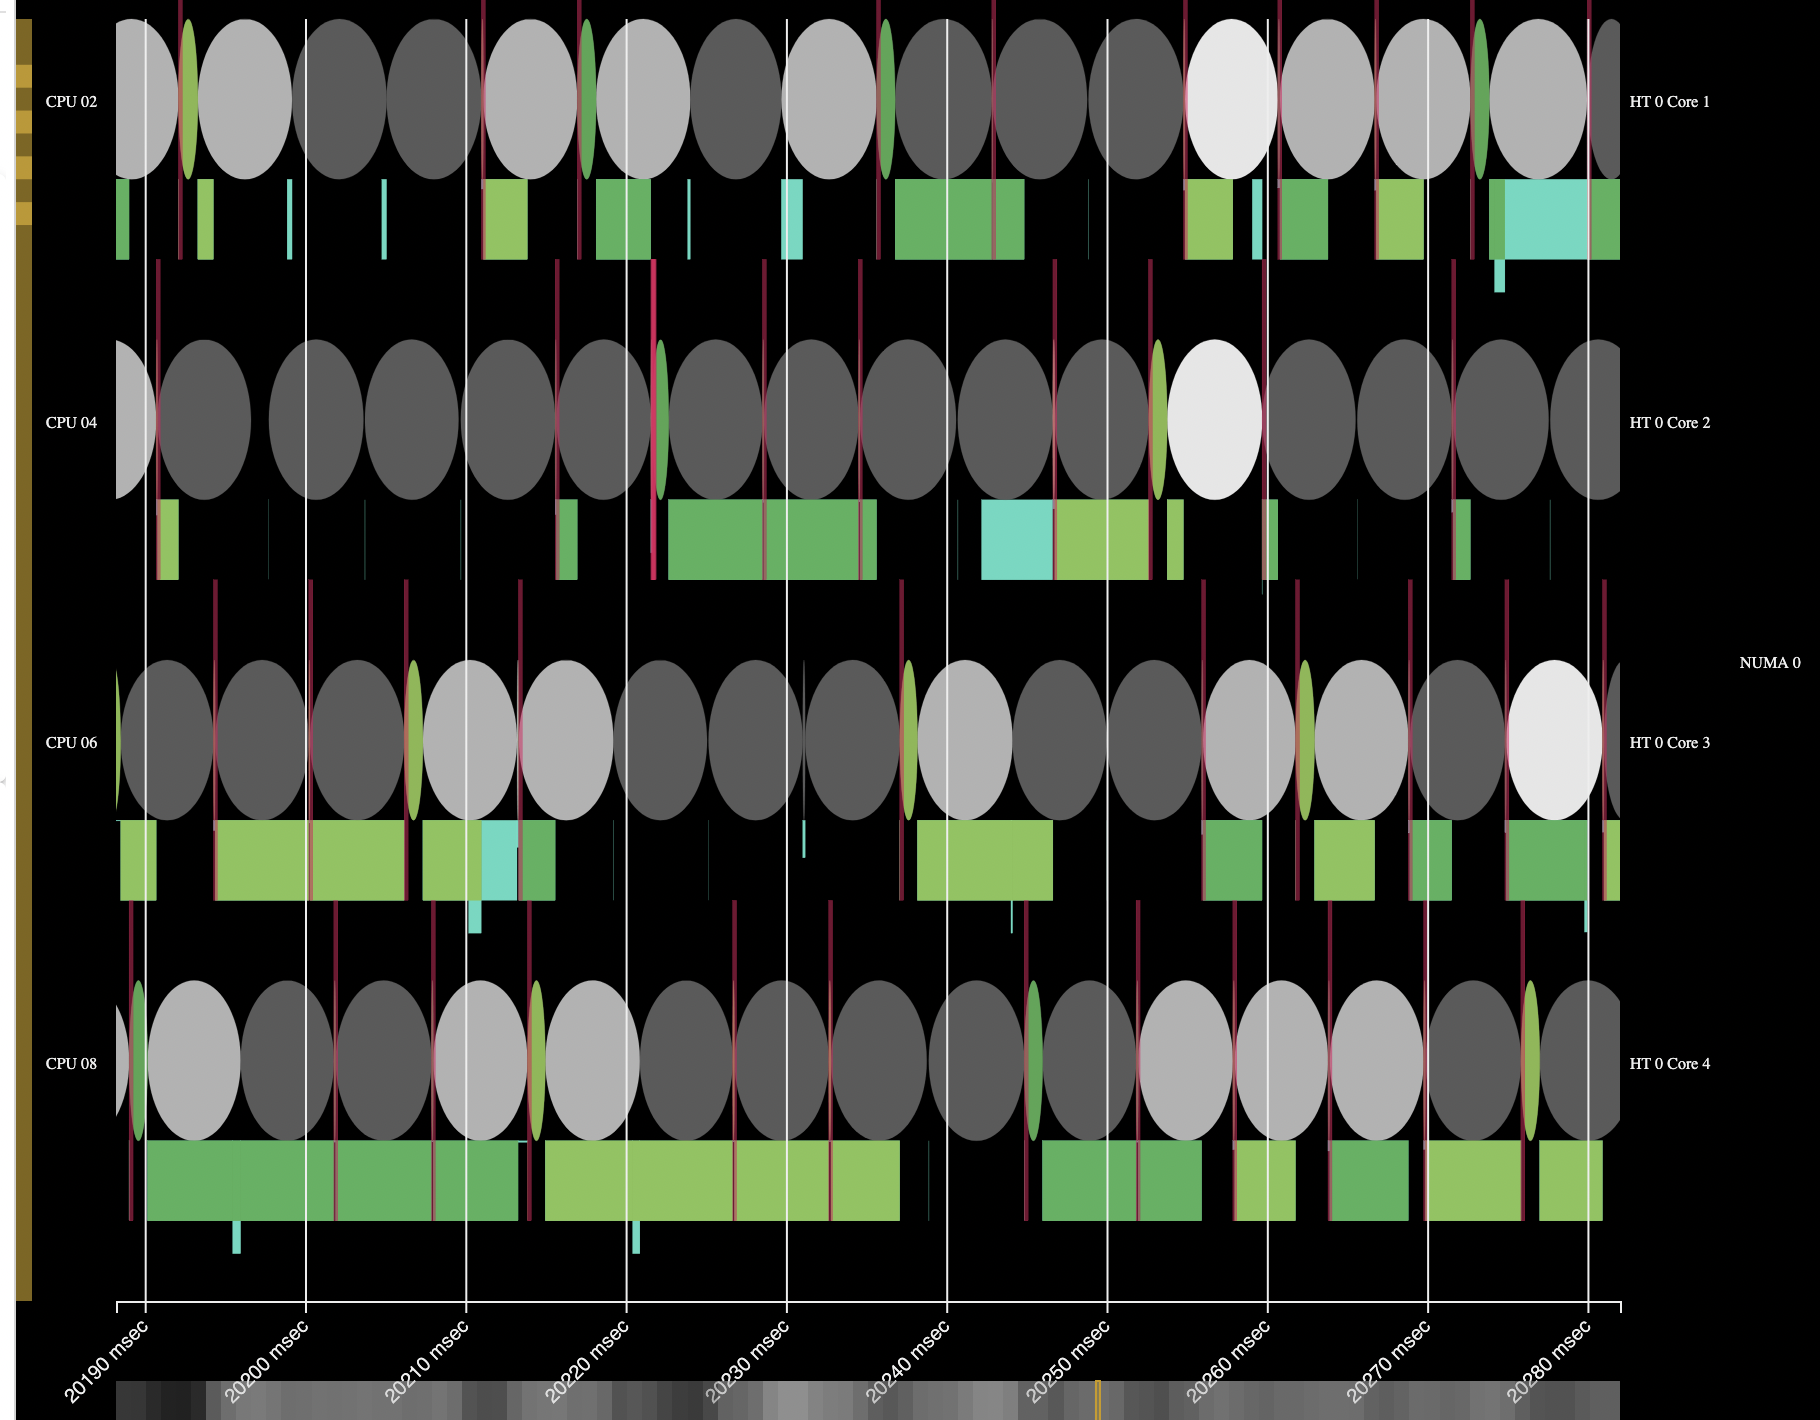
\includegraphics[width=\columnwidth]{graphs/schedviz-schedbe.png}
    \caption{The BE threads are colored in two different shades of green, the LC
    threads are the grey ones, the red vertical lines are the scheduler
    initially choosing a BE thread, which leads to an attempt to steal a queued
    LC one. As a result, BE threads only run when there are no queued LC
    threads.}\label{fig:schedviz-schedbe}
\end{figure}

We start by running the microbenchmark experiment using \schedbe{}. We use the
\cgroups{} interface to set the BE workloads to be marked as idle via the
\cgroups{} api, except that with the modified kernel that now puts the BE tasks
in \schedbe{}. We can see the resulting performance in
\autoref{fig:srv-bg-schedbe}. As desired the latency of the server remains
stable after the background tasks start. This does not mean that the background
task never runs: the lower graph still shows iterations of image resizing being
done. The difference is that now the background tasks will reliably get
interrupted when the LC server has a request to process. We can see this
happening in an outtake of the schedviz visualization for one of the runs in
\autoref{fig:schedviz-schedbe}. The green BE processes run only in the gaps
where there is no queued LC process, and are immediately preempted when one
wakes up, on whatever core that may be. The red lines show when the core has
chosen intially to run a BE process, sometimes followed by an LC process that
was stolen as a result running next, sometimes by the BE process actually
running because there was no queued LC thread to steal.

\begin{figure}[t]
    \centering
    \begin{subfigure}[t]{0.49\columnwidth}
        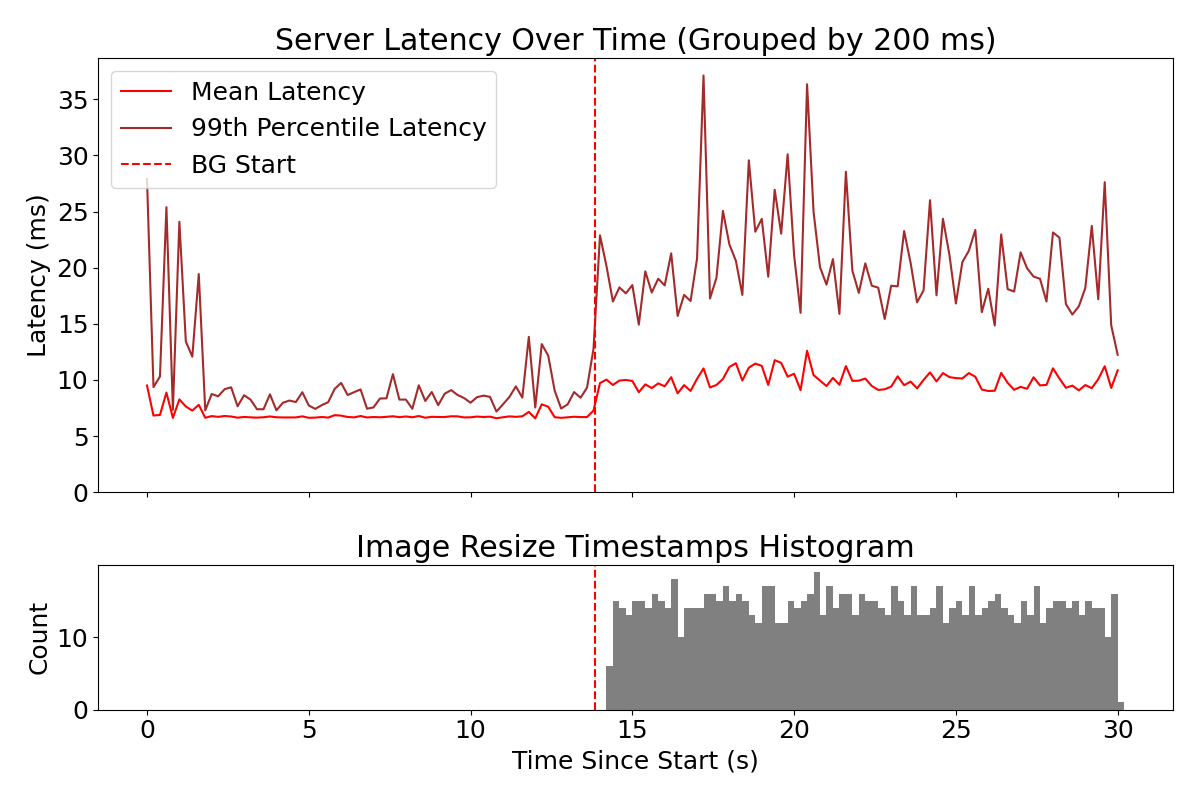
\includegraphics[width=\columnwidth]{graphs/kubernetes-idle.png}
        \caption{BE running as \schedidle{}}\label{fig:kubernetes-idle}
    \end{subfigure}
    \hspace{\fill}
    \begin{subfigure}[t]{0.49\columnwidth}
        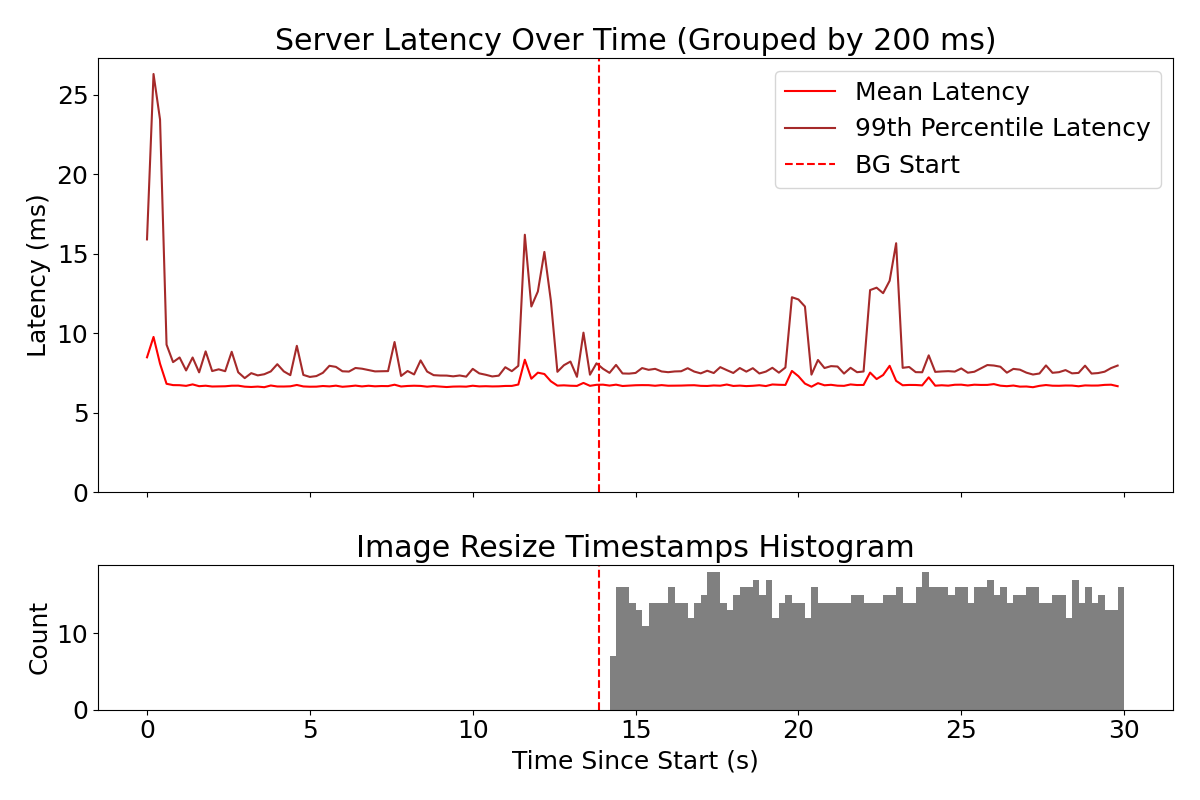
\includegraphics[width=\columnwidth]{graphs/kubernetes-schedbe.png}
        \caption{BE running as \schedbe{}}\label{fig:kubernetes-schedbe}
    \end{subfigure}
    \vspace{4pt}
    \caption{The same experiment as in \autoref{fig:kubernetes-unedited}, but
    running the BE as a \schedidle{} and a \schedbe{} task}\label{fig:kubernetes-other}
\end{figure}

We also run the Kubernetes application from \autoref{fig:kubernetes-unedited}
using \schedidle{} as well as \schedbe{}. The results are in
\autoref{fig:kubernetes-other}, we can see that, as above, \schedidle{} regains
some of the performance in comparison to the default weight-based isolation, but
still shows an influence on the LC web application by the BE image resize job.
\schedbe{} completely gets rid of the gap, and we can see that the latency
profile os the web application is exactly the same before and after starting the
image resize job.


\subsection{Is parking necessary?}

Linux in its current form safeguards heavily against any form of starvation. As
we saw earlier, real time Fifo applications have strict priority and thus
represent a possible antagonist that would be able to starve everything else.
However, Linux has two different safe guards that protect against this. One is
that Fifo is as a scheduling class rate-limited: there are tuneable parameters
at \texttt{/proc/sys/kernel/sched\_rt\_runtime\_us} and
\texttt{/proc/sys/kernel/sched\_rt\_period\_us}, that together define a rate
limit for the Fifo class as a whole. The failsafes go further than just that
though: even when set to be equal (ie Fifo gets the full runtime each period if
it wants), the Normal scheduling class also has a so-called \textit{deadline
server}, which is basically a process is in the Deadline scheduling class with a
small amount of runtime per period~\cite{lkml-deadline-srv}. This deadline
server is in essence a representative of the Normal scheduling class, and when
the Deadline scheduler runs the server, that hands control over to the Normal
scheduler, which picks a thread to run.
% https://lore.kernel.org/lkml/20200807095051.385985-5-juri.lelli@redhat.com/ 


\begin{figure}[t]
    \centering
    \begin{subfigure}[t]{0.49\columnwidth}
        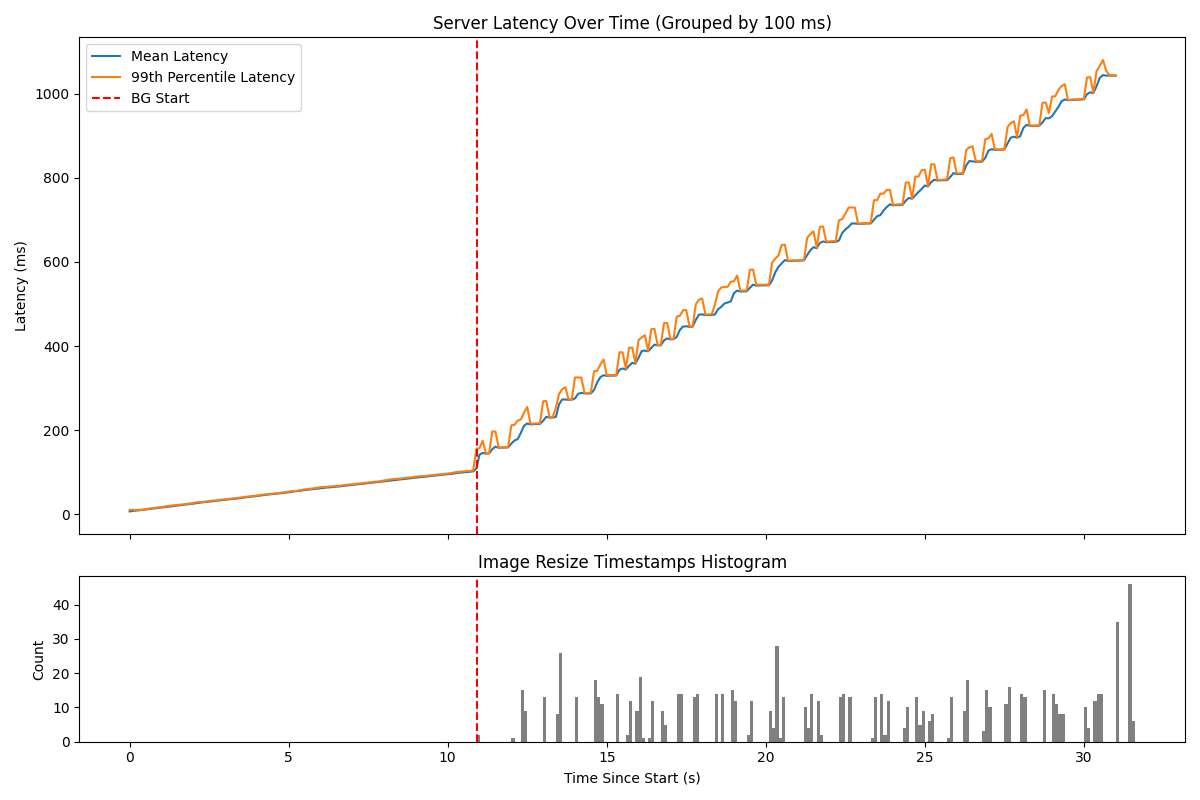
\includegraphics[width=\columnwidth]{graphs/overload-rt.png}
        \caption{LC in real time, throttling}\label{fig:overload-rt}
    \end{subfigure}
    \hspace{\fill}
    \begin{subfigure}[t]{0.49\columnwidth}
        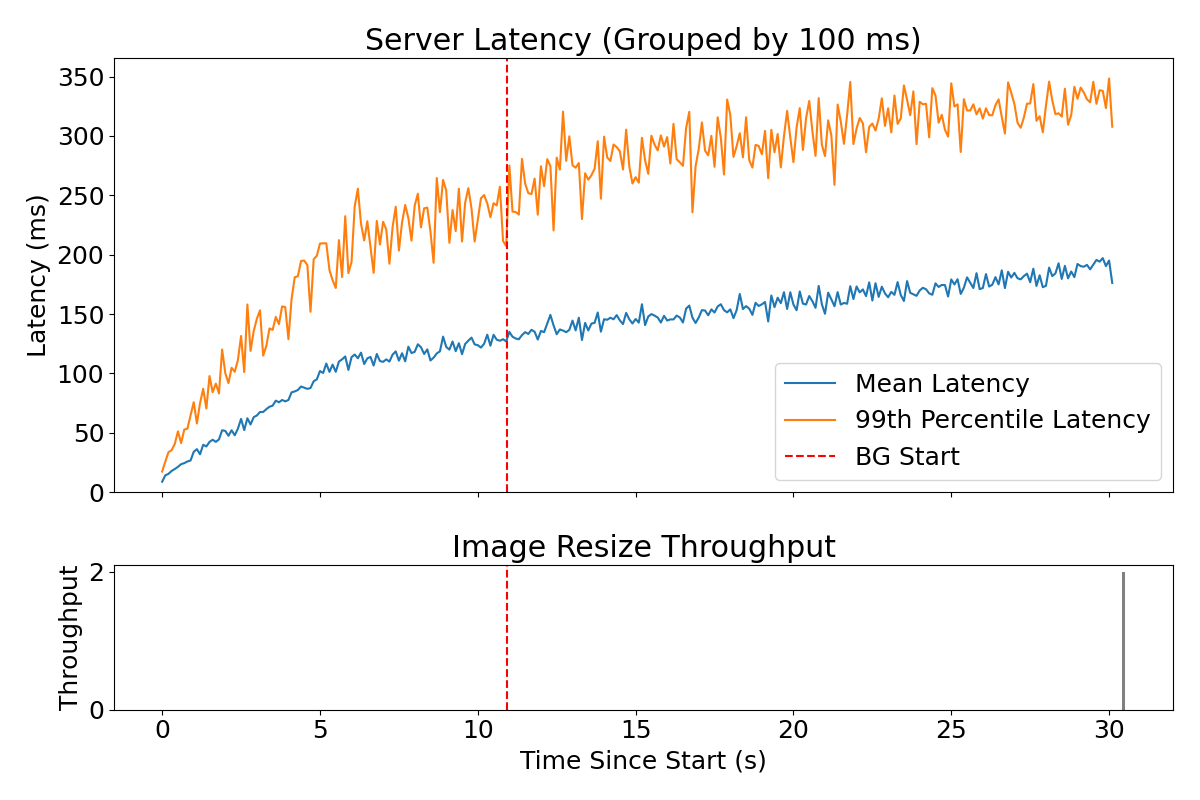
\includegraphics[width=\columnwidth]{graphs/overload-schedbe.png}
        \caption{BE in \schedbe{}, no throttling}\label{fig:overload-schedbe}
    \end{subfigure}
    \vspace{4pt}
    \caption{throttling the LC server under extremely high utilization, vs
    letting it starve the BE userspace processes}
\end{figure}


We can see this in action if we turn up the utilization on the real time
experiment: we run it so that the baseline utilization is oversaturated (100\%),
the results are in \autoref{fig:overload-rt}. We see spikes begin to
appear after starting the BE task. This is because the Fifo server gets
throttled in favor of running the BE tasks; we see parallel spikes where the
background tasks are allowed to run. Notice also the increase of the slope of
response times after starting the background tasks: the deadline server
mechanism only kicks in if there is load to run, so once it does the resulting
throttling degrades the servers performance signigicantly. If this were taking
place during a load spike while waiting for new server instances to start, the
presence of BE load would significantly impact the queue length/performance
degradation while the new server starts up.

On the other hand, we see in \autoref{fig:overload-schedbe} what happens
if, in that same experiment, \schedbe{} allows the BE userspace process to be
parked. Notice that the BE does not make progress until the very end, when the
server is done processing the requests (the experiment stops the client after 30
seconds and the server from then finishes the backlog of requests).



\subsection{Cost of \schedbe{}}

We evaluate the cost of the additional checks required by \schedbe{} by looking
at how long the code takes to run, and how much lock contention it creates.